
\chapter{Tags}\label{tags_chapter}
\minitoc 
\section{Tagging surfaces with ISE-MeshTools.}
25 tags (ordered between 0 and 24) can be given
a label, a color, a transparency, and be manually
delimitated. A greater number of tags can be given
to a surface using automatic tagging tools such as the ``Tag connected regions" tool, but these
additionnal tags can not be labeled or manually edited. As stated earlier, in order to edit tags, it is advisable to activate the ``tag mode" (press ``
\includegraphics[scale=0.7]{images/pixmap/Tag_select_mode.png}" button). In this mode, selected surfaces (on which you can interact and tag) can be drawn according to tag values at each vertex if ``tag display mode"is active. Press ``
\includegraphics[scale=0.7]{images/pixmap/Show_Tag_Window.png}" to activate ``tag diplay mode". When active, the tag color scale shows up in the bottom-right part of the 3D rendering window (see Fig. \ref{tag_color_scale}). Selected surfaces can be tagged using the pencil tag tool (``
\includegraphics[scale=0.7]{images/pixmap/pencil.png}"), the magic wand tag tool ( ``
\includegraphics[scale=0.7]{images/pixmap/magic_wand.png}"), the paint bucket tag tool (``
\includegraphics[scale=0.7]{images/pixmap/Flood_fill.png}") or the lasso tag tool (``
\includegraphics[scale=0.7]{images/pixmap/Lasso_plus.png}").

\begin{figure}
  \centering
  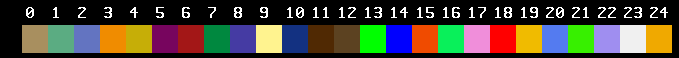
\includegraphics[scale=0.5]{images/Tags/Tag_color_scale.png} 
	\caption{Example of tag color scale}
\label{tag_color_scale}
 
\end{figure}



\subsection{Pencil tag tool}

\includegraphics[scale=0.7]{images/pixmap/pencil.png}\\
\textbf{Pencil tag tool controls:}\\
T pressed + left mouse click : tags the selected surface using currently active tag.\\
T pressed + right click : tags the selected surface using tag 0 (usually used as ``exterior" tag). This option is often used to ``clear" a wrongly tagged part.\\
\textbf{Pencil tag special option:}\\
\noindent
\begin{minipage}{0.6\textwidth}
pencil tag size can be modified in the Tag option window. This
option defines the tag propagation extension level, which starts at
the vertex on which the mouse click is performed.
\end{minipage}    
\begin{minipage}{0.4\textwidth}\centering
  
\includegraphics[scale=0.5]{images/Tags/Pencil_tag_size.png}
 \captionof{figure}{Pencil tag size option}
 \end{minipage} 
\noindent



\subsection{Magic wand tag tool}

\includegraphics[scale=0.7]{images/pixmap/magic_wand.png}\\
\textbf{Magic wand tag tool controls:}\\
T pressed + left mouse click : tags the selected surface using currently active tag.
T pressed + right click : tags the selected surface using tag 0 (usually used as ``exterior" tag). This option often is used to ``clear" a wrongly tagged part.\\
\\
\noindent
\textbf{Magic wand special option:}\\
\noindent
\begin{minipage}{0.6\textwidth}
Magic wand limit angle size can be modified in the Tag option window.
\end{minipage}    
\begin{minipage}{0.4\textwidth}\centering
  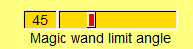
\includegraphics[scale=0.5]{images/Tags/Magic_wand_options.png}
 \captionof{figure}{Magic wand limit angle}
 \end{minipage} 
\noindent
 This option defines the tag propagation extension level, which starts at the vertex on which the mouse click is performed : propagation stops if the angle between the notmal of current vertex and the normal of the vertex on which the mouse click was done is found is greater than the defined
angle.



\subsection{Paint bucket tag tool}

\includegraphics[scale=0.7]{images/pixmap/Flood_fill.png}\\
\textbf{Paint bucket tag tool controls:}\\
T pressed + left mouse click : tags the selected surface using currently active tag.\\
T pressed + right click : tags the selected surface using tag 0 (usually used as ``exterior" tag). This option is often used to ``clear" a wrongly tagged part.\\ 
Note : the paint bucket tag tool works exactly like the magic wand tag tool when the magic wand limit angle is set to 180\degree.

\subsection{Pencil tag, magic wand and paint bucket common option}
\noindent
\textbf{Magic wand special option:}\\
\noindent
\begin{minipage}{0.6\textwidth}
These 3 tools share a common option, available in the Tag option
window, the ``allow color override" checkbox.\end{minipage}    
\begin{minipage}{0.4\textwidth}\centering
  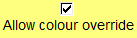
\includegraphics[scale=0.5]{images/Tags/Allow_color_override.png}
 \captionof{figure}{Allow color override option}
 \end{minipage} 
\noindent
- If checked : no attention is paid to the color of the vertex on
which the left/right click was done during tag propagation.\\
- If unchecked: tag propagation will stop if a tag color different from 0 (exterior tag) and from that of the vertex on which the mouse click was done is found.\\
\textbf{Important note:} be careful when using ``allow color override" option \underline{checked} with the paint bucket tag tool or with the magic wand, as it will paint a large region uniformly (minutes or even hours of work may be lost in a single click, if you did not save your tagged surface in .vtk format earlier).

\subsection{Lasso tag tool} \label{lasso_tag_section}

\includegraphics[scale=0.7]{images/pixmap/Lasso_plus.png}\\
The lasso tag tool can be used alone (option 1) or in combination with the pencil, the magic wand or the paint bucket (option 2). Once ``lasso tag tool" button is pressed, the mouse cursor changes to a cross in the 3D window. Additional mouse and keyboard controls become available (see Table \ref{lasso_tag_controls}). Once option 1 or option 2 is achieved, the usual mouse and keyboard controls become available
again.

\begin{table}
\begin{tabularx}{\linewidth}{ | X | X | }
\hline			
Left click & Adds a segment to polygon (segments are drawn yellow) \\ \hline			

Right click & Connects last segment to first segment. If two segments cross each other, lasso tag action is cancelled. Otherwise, the closed polygon is drawn red.\\ \hline			

Option 1: once polygon is closed, middle click or ``C" + right click. & when the click falls \textbf{inside}/\textit{outside} the closed red
polygon: the region falling \underline{inside} the polygon
\textbf{is tagged}/\textit{is not tagged} using the active tag
color, respectively. The region falling \underline{outside}
the polygon \textbf{is not tagged}/\textit{is tagged} using the
active tag color, respectively.

\\ \hline			
Option 2: once polygon is closed: Press ``T" + left or Press ``T" +right click  & The selected tag tool (magic wand or paint bucket) is be used, but tag propagation will not
cross over polygon edges.
\\ \hline	
		

\end{tabularx}
\caption{Lasso tag controls}	
\label{lasso_tag_controls}	
\end{table}

\section{Show tag options window.}

The ``Tag options" window (see Fig. \ref{tag_options_window}) can also be opened by clicking on ``
\includegraphics[scale=0.7]{images/pixmap/Show_Tag_Window2.png}" .
\begin{figure}
  \centering
  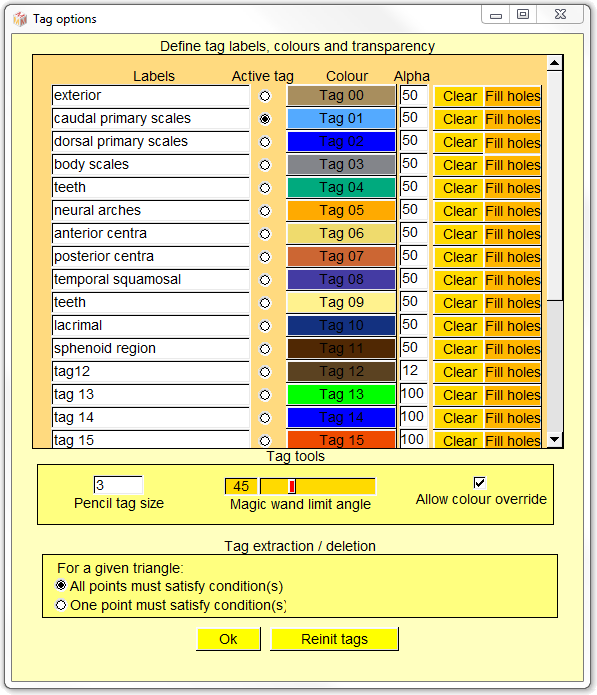
\includegraphics[scale=0.5]{images/Tags/Tags.png} 
	\caption{Tag options window.}
\label{tag_options_window}
 
\end{figure}
\noindent
\textbf{Available controls:}\\
\\
\noindent
\textit{\underline{Define tag labels, colors and transparency group:}}\\
\textit{Labels:} you may define tag labels for all 25 available tags.\\
\textit{Active tag:} you may define the currently active tag.\\
\textit{color}: you may define the color for all 25 available tags.\\
\textit{Alpha:} you may define the transparency for all 25 available tags.\\
\textit{Clear:} clears the tag region (all vertices of this region will be set to 0 = Tag 00).
\textit{Fill holes:} opens the ``Fill holes" window (see Fig. \ref{fill_holes_window}). Pressing ok will fill all regions adjacent to the concerned tag region (Tag id) containing less than ``Max num" vertices (see for instance Fig. \ref{tag_fill_holes_example}).
\begin{figure}
  \centering
  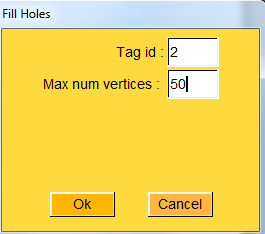
\includegraphics[scale=0.5]{images/Tags/Fill Holes.png} 
	\caption{Fill Holes window.}
\label{fill_holes_window}
 \end{figure}

\begin{figure}
  \centering
  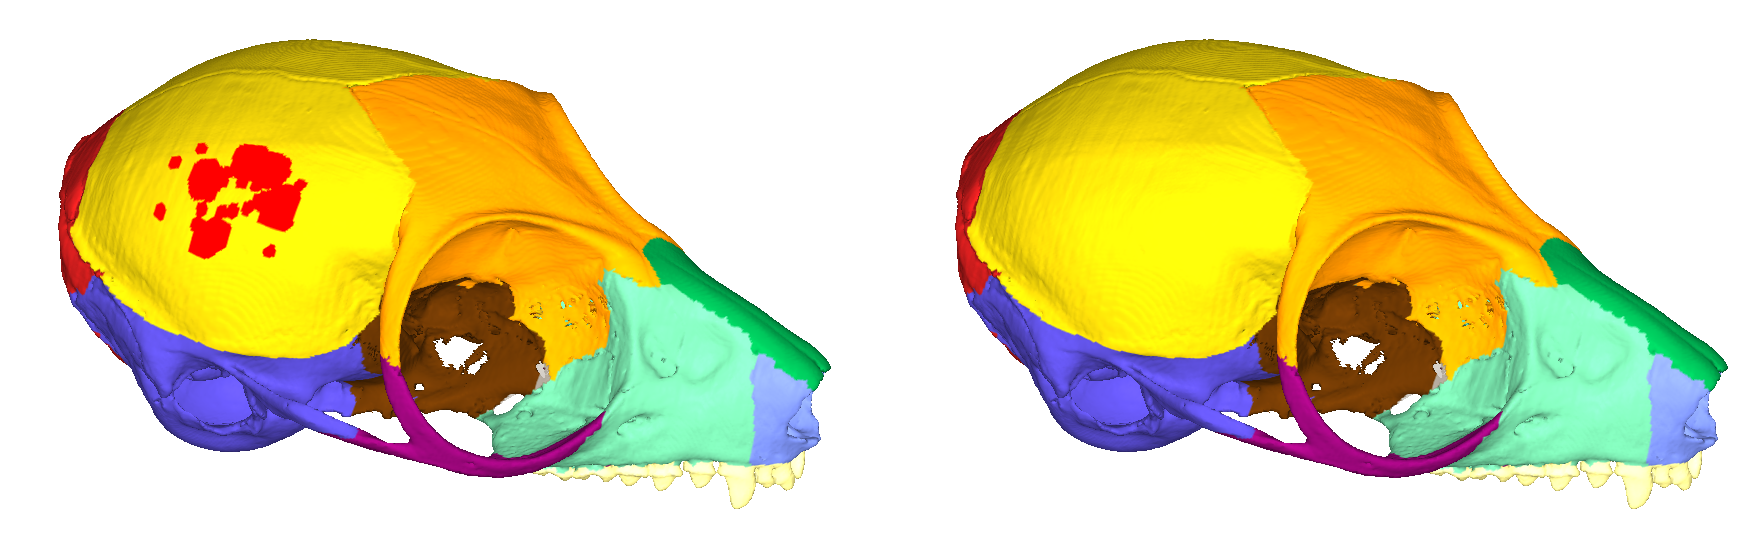
\includegraphics[scale=0.25]{images/Tags/Fill_holes2.png} 
	\caption{Example of tag hole filling. Left : cranium of \textit{Microcebus murinus} presenting a parietal region tagged mostly in yellow, and presenting red ``holes". Right : ``holes" present in the yellow region were filled using ``Max num vertices" = 4000 option.
}
\label{tag_fill_holes_example}
 \end{figure}
\noindent
\textit{\underline{Tag tools group:}}
\textit{Pencil tag size:} This option defines the tag propagation extension
level of the pencil tag tool. Magic wand limit angle : This option defines the tag propagation extension level of the magic wand tag tool (see above for further explanations).\\
\textit{Allow color override:} The pencil, magic wand and paint bucket tag tools share this option. If active, tag propagation will stop if a tag color different from 0 (exterior tag) and from that of the vertex on which the mouse click was done is found.\\
\\
\noindent
\textit{\underline{Tag extraction/deletion:}}\\
For a given triangle : \textit{All points must satisfy condition} / \textbf{One point must satisfy condition.} This option defines the extent to which region extraction or deletion is performed at the boundaries of the concerned tagged region.\\\\
\noindent
Example of tag merging. Left : cranium of \textit{Microcebus murinus} presenting the parietal region
tagged in yellow, the frontal region tagged in orange. Right : frontal tag region was merged into the parietal region.


\section{Convert RGB colors to Tags.}

This option (see Fig. \ref{rgb_conversion}) may be useful when you just have opened a .ply file already containing RGB colors (for instance, let us suppose that you have painted a surface using MeshLab software, and that you wish to convert those colors into tags). RGB colors contained in .ply files are inserted inside the RGB scalar when opened with MeshTools. I you plan to transform those RGB values into tags with MeshTools, be aware of the fact that RGB scalar is reinitialised extremely frequently: for instance as soon as you activate the tag or the scalar display mode, or whenever you change the objects' color rendering. So I advise you to use the present option only immediately after opening the surface.
\begin{figure}
  \centering
  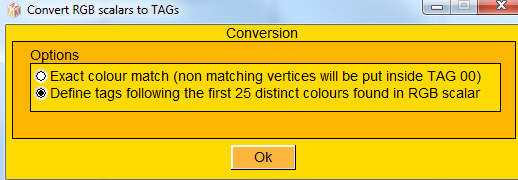
\includegraphics[scale=0.5]{images/Tags/Convert.png} 
	\caption{Convert RGB scalars to TAGS window}
\label{rgb_conversion}
\end{figure}
You have two options :\\
\textbf{\underline{1) exact color match}}\\
$\rightarrow$ In that case, in order to be given a tag value other than Tag 00, a vertex must satisfy the following condition: its RGB scalar value should match one of the 25 colors defined in the ``Tags options" window. If a vertex does not satisfy this condition, it is given the Tag 00 value.\\
\textbf{\underline{2) Define tags following the first 25 distinct colors found in RGB scalar}}\\
$\rightarrow$ In that case the following sequence of operations is applied:\\
a) ISE-MeshTools searches for the first 25 distinct RGB colors inside the object; ISE-MeshTools gives them numbers ranging from 0 to 24. Important : if more than 25 distinct colors exist in the RGB scalar, they are not given a tag value.\\
b) ISE-MeshTools updates tag colors according to the 25 first colors found in the RGB scalar.\\
c) All vertices are given a Tag value following the procedure defined above in \#1 (exact color match).\\
Advantages of \#1 : if you have well prepared your RGB colors so that they matches well those associated with the 25 tags, this procedure will work perfectly.\\
Advantages of \#2 : if you have up to 25 distinct RGB colors in your .ply file and if you do not want to bother to edit manually the 25 tags and give them a RGB color, you will save time with this procedure. 
\\Drawbacks of both methods: if your file contains more than 25 distinct RGB colors, you will definitely lose information in the process.
\\Be also aware that when saving .ply files with ISE-MeshTools, the RGB coulours saved within the file are those currently rendered in the 3D screen. If you spent time to color a 3D surface in .ply format (for instance with MeshLab) and you have opened it subsequently with ISE-MeshTools and have saved it again, there is a high probability that all the initial RGB colors will have been replaced with those rendered in ISE-MeshTools.


\section{Merge tags.}
\noindent
\begin{minipage}{0.5\textwidth}
Two tagged regions can be merged into a single one
All source tags will be put into target tags.
\end{minipage}    
\begin{minipage}{0.5\textwidth}\centering
  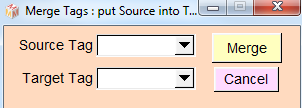
\includegraphics[scale=0.5]{images/Tags/Merge_tags.png}
 \captionof{figure}{Merge tags window}
 \end{minipage} 
\noindent
\begin{figure}
  \centering
  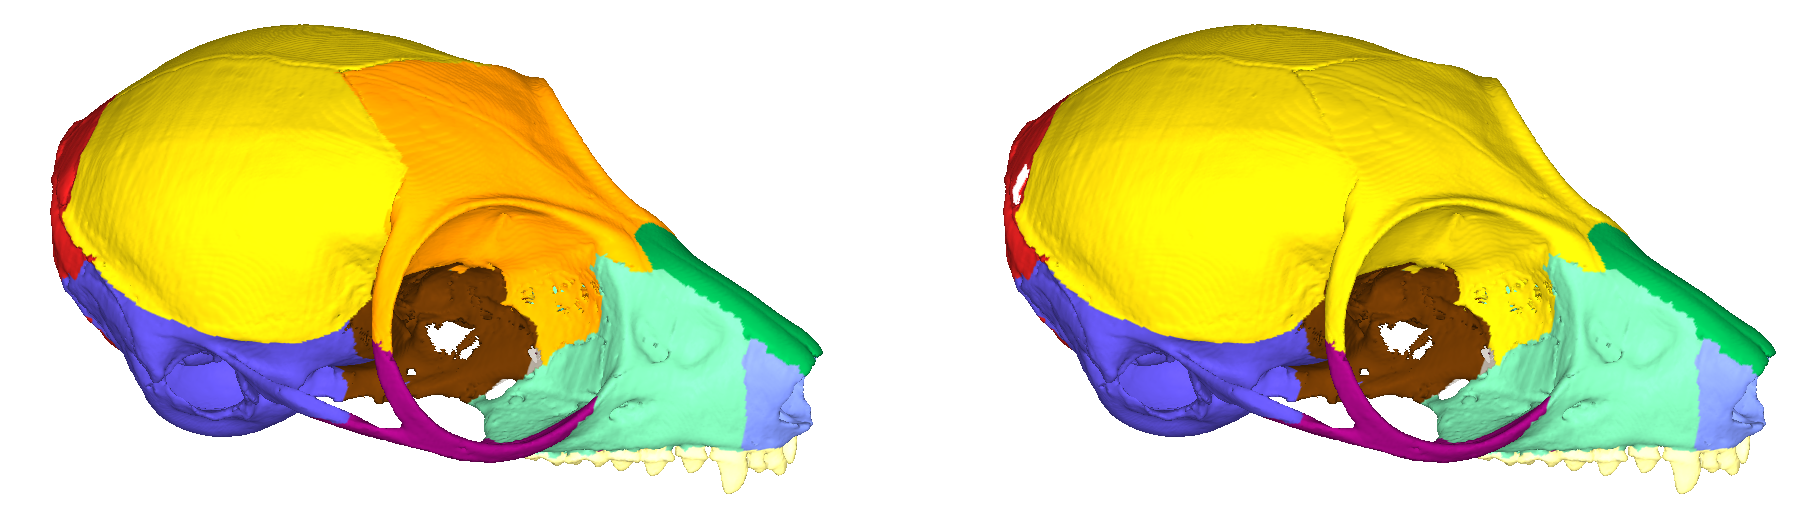
\includegraphics[scale=0.25]{images/Tags/Merge.png} 
	\caption{Example of tag merging. Left : cranium of \textit{Microcebus murinus} presenting the parietal region
tagged in yellow, the frontal region tagged in orange. Right : frontal tag region was merged into
the parietal region.}
\label{merge_tags}
 
\end{figure}



\section{Tag connected regions.}
This option implies vtkPolyDataConnectivityFilter. This filter will tag all non-connected regions of the
selected input surface into different colors (see Fig. \ref{tag_connected}).
\begin{figure}
  \centering
  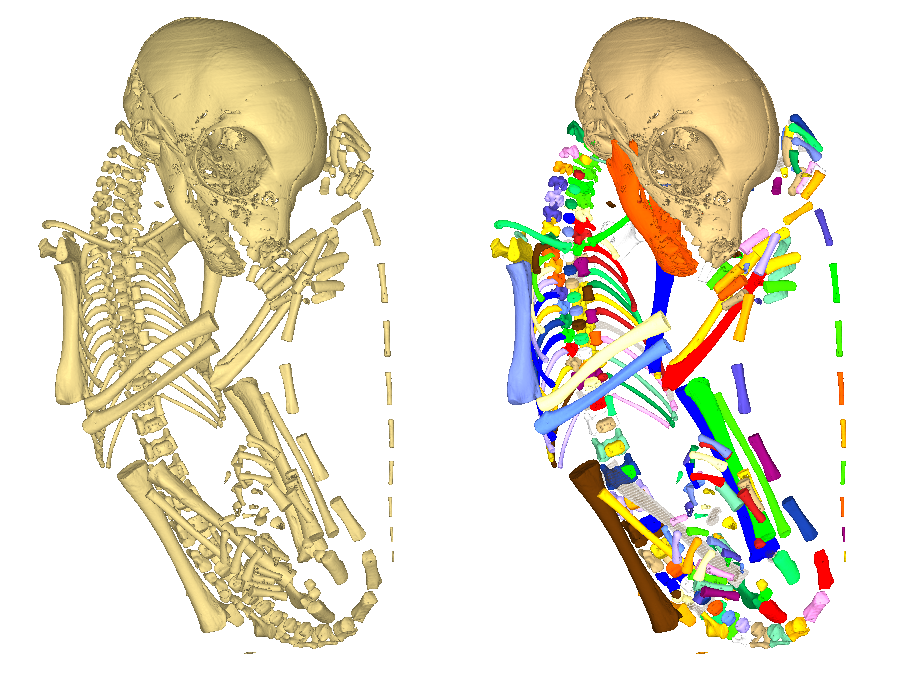
\includegraphics[scale=0.45]{images/Tags/Lemur_tag_input_output.png} 
	\caption{Left: original surface. Right: the same mesh automatically tagged into 304 non connected regions.}
\label{tag_connected}
 
\end{figure}



\section{Extract.}


Note: The ``Tag extraction/deletion" option in the Tag options window will affect the boundaries of
the extracted regions (see Fig. \ref{tag_extraction}).

\begin{figure}
  \centering
  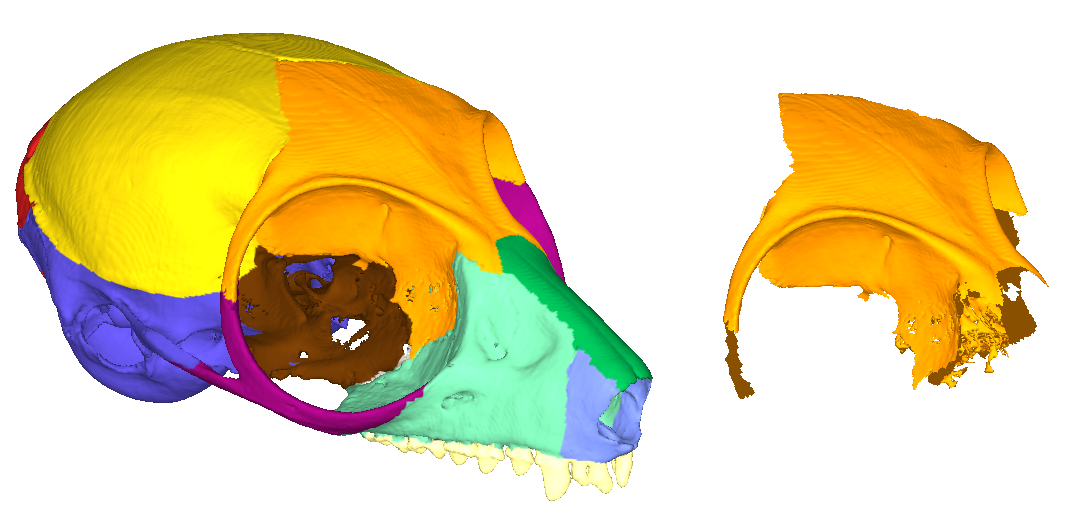
\includegraphics[scale=0.35]{images/Tags/Extract_tag.png} 
	\caption{Example of tag extraction. Left : cranium of \textit{Microcebus murinus} presenting the frontal region
tagged in orange. Right : frontal tag region was extracted into a new surface object.}
\label{tag_extraction}
 
\end{figure}



\subsection{Extract active tag corresponding region}
Using this window, a single mesh will be created out of the active tag corresponding region of the
selected object. 

\subsection{Extract all tagged regions as several new objects}
\noindent
\begin{minipage}{0.5\textwidth}
Using this window (see \ref{extract_all_window}), all meshes will be created out all different existing tags. In order to prevent extremely small surface objects to be created, a minimal region size parameter for tag extraction is asked. For an example, see Fig. \ref{extract_all}.\end{minipage}    
\begin{minipage}{0.5\textwidth}\centering
  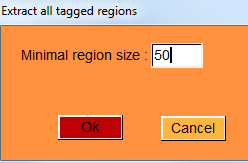
\includegraphics[scale=0.5]{images/Tags/Extract_all_tagged_regions.png}
 \captionof{figure}{Extract all tagged regions window.}
\label{extract_all_window}

 \end{minipage} 
\noindent
\begin{figure}
  \centering
  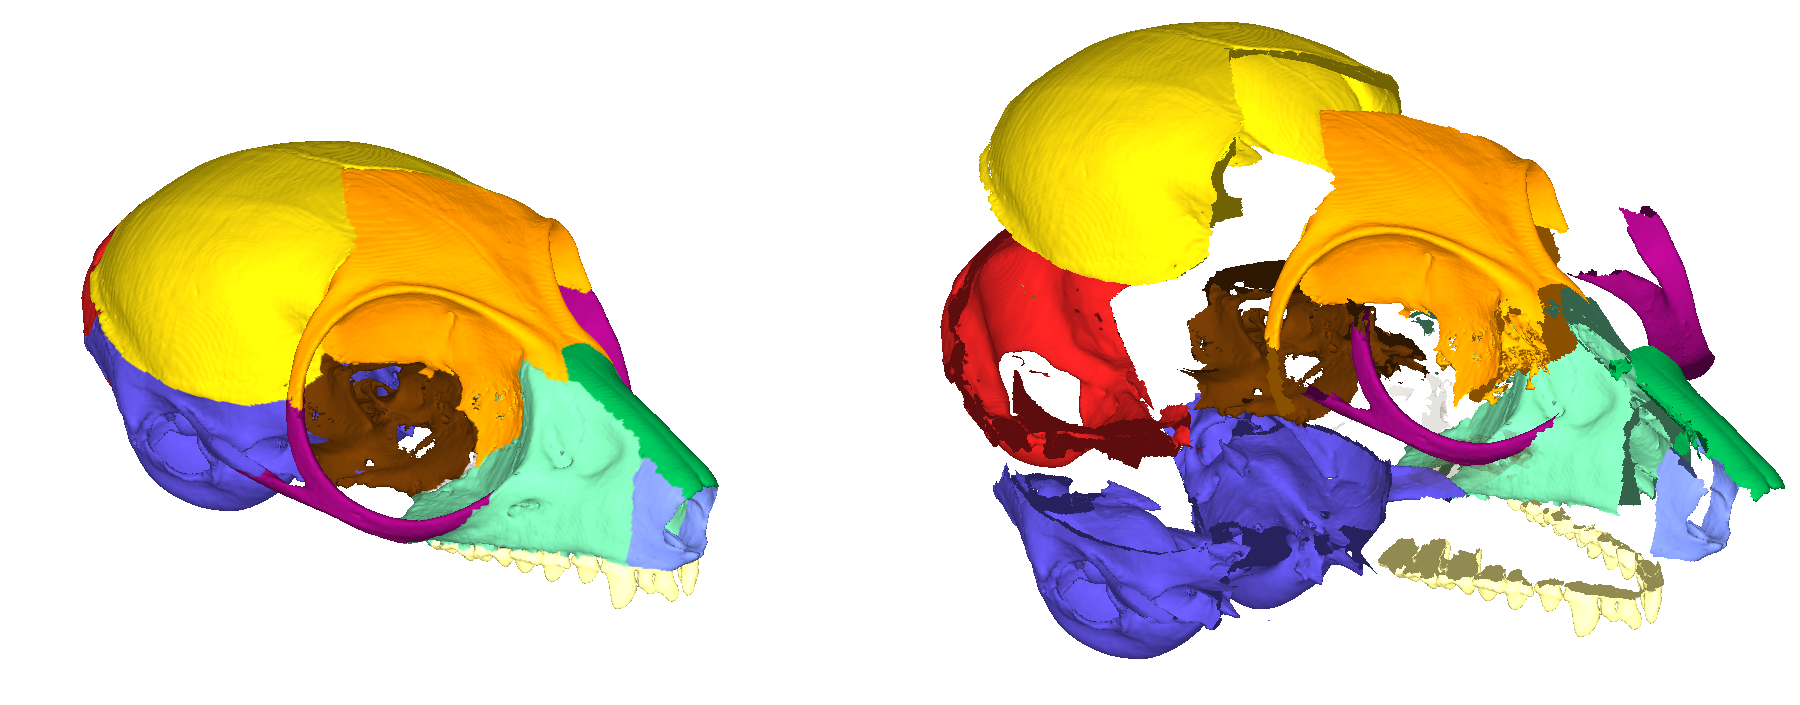
\includegraphics[scale=0.25]{images/Tags/Extracted_tag2.png} 
	\caption{All tags extraction. Left: original tagged surface. Right: all tagged regions were extracted into single independent surface objects}
\label{extract_all}
 
\end{figure}

\subsection{Extract one tagged region as 1 new object}
\noindent
\begin{minipage}{0.5\textwidth}
This option works similarly as the ``Extract active tag
corresponding region" option mentioned above, except that
you can reach tag id values beyond the 25 reachable in the
Tag options window.
\end{minipage}    
\begin{minipage}{0.5\textwidth}\centering
  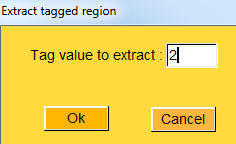
\includegraphics[scale=0.5]{images/Tags/Extract_one_tagged_region.png}
 \captionof{figure}{Extract tagged region window.}


 \end{minipage} 
\noindent



\subsection{Extract tag or other scalar range as 1 new object}
\noindent
\begin{minipage}{0.5\textwidth}
Using this option, you may extract several tagged regions
into one single mesh, or all regions ranging from a minimal
value up to a maximal value for a given scalar into a single
new mesh. See for instance Fig. \ref{extract_scalar_range}.
\end{minipage}    
\begin{minipage}{0.5\textwidth}\centering
  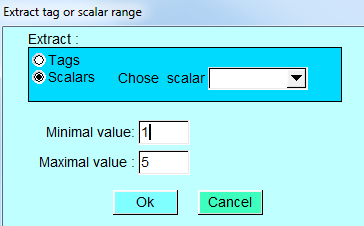
\includegraphics[scale=0.5]{images/Tags/Extract_scalar_range.png}
 \captionof{figure}{Extract scalar range window.}
 \end{minipage} 
\noindent

\begin{figure}
  \centering
  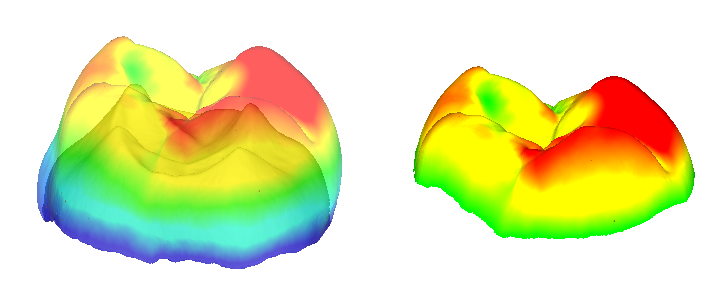
\includegraphics[scale=0.6]{images/Tags/Extract_range.png} 
	\caption{Extraction of the region showing an enamel thickness greater than 1 mm. Specimen : enamel surface of SP07 specimen (see ``Scalars" and ``Acknowledgement" sections for details regarding this specimen). Image credit : Mona Le Luyer (PACEA, Bordeaux).}
\label{extract_scalar_range}
 
\end{figure}



\section{Delete.}

Note: The ``Tag extraction/deletion" option in the Tag options window will affect the boundaries of the deleted regions.
\subsection{Delete one tagged region}
\noindent
\begin{minipage}{0.5\textwidth}
This option works similarly as the ``Extract one tagged
region" option mentioned above, except that it deletes the
selected tag region.
\end{minipage}    
\begin{minipage}{0.5\textwidth}\centering
  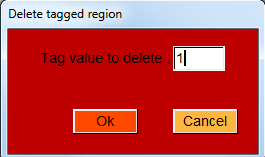
\includegraphics[scale=0.5]{images/Tags/Delete_one_tagged_region.png}
 \captionof{figure}{Delete tagged region window.}
 \end{minipage} 
\noindent




\subsection{Delete active tag corresponding region}
This option works similarly as the ``Extract active tag corresponding region" option mentioned above, except that it deletes the corresponding active tag region.

\subsection{Delete all tagged regions except TAG 00}
This option deletes all tagged region except the vertices tagged with TAG 00 (exterior).